\setcounter{chapter}{2} 

\chapter{Lightning}
Observation of lightning is a  natural part of human history, from early man believing it to be wrath of deities, to the modern storm chaser utilizing radar observations of precipitation to get the best view of a storm. The study of this phenomenon on the other hand is relatively new. The first steps in this endeavour was the experiments performed by Benjamin Franklin, along with the development of the theory of electromagnetism. Only in the last century have we acquired the means to thoroughly investigate the electrical and meteorological mechanisms resulting in a thunderstorm. This is due to both more available measurements and better physical understanding. The measurements are made possible by aircraft being able to fly through storm clouds providing in-situ observation, and satellite imaging providing a view into the vertical composition and structure of a cloud.

\section{Convection and the nature of clouds}

Instability can be understood by recognizing that warm air is less dense than cold air, thus being buoyant in the colder surrounding air. When air rises, less pressure is exerted on it, since the atmosphere is densest at the surface. This lower pressure causes work to be done by the rising air, to expand to a new equilibrium. If the air rises fast enough for the expansion to be adiabatic, this work leads to a cooling of the air mass. This cooling slows the vertical movement due to less buoyancy.

However if moisture is present at the surface water vapor will be displaced upwards by this vertical movement. When the air mass is cooled by the expansion, the saturation vapor pressure decreases. Lower saturation vapor pressure favours more water in the condensed phase, either as ice or water particles . Condensation of water vapor heats the ascending air, which causes more vertical movement. Thus a dry atmosphere is inherently more stable than a humid atmosphere, as the lack of condensation would lead to equilibrium due to adiabatic cooling.

If temperatures are sufficiently low ($\leq 0 ^{\circ} C$) the liquid water may freeze to ice crystals. The uncertainty here is due to the immense heat released when a crystalline surface is created, such that a typically sized liquid droplet requires a temperature of around $\leq \approx-38 ^{\circ} C$ to initiate homogeneous freezing. Alternatively, by introducing a surface which the structure can grow on (here an ice nucleation particle), this reduces the energy released, thus raising the temperature requirement for freezing (\cite{jeffery1997}). This leads to relatively clean air containing super-cooled liquid droplets (below bulk freezing temperature of $0 ^{\circ} C$).

\section{Natural Lightning}
There are different theories in the still open field of thunderstorms, pertaining to both the electrification mechanisms and the general electrical structure. This is further complicated by the fact that there seems to be different mechanisms at work for different scales of storms.

The \textit{typical} lightning storm is created in summertime. It can generally be caused by solar radiation heating up the ground, and creating an unstable atmosphere (\cite{rakovBok}). Alternatively, or in combination with the aforementioned effect, this instability may be caused by very cold air moving over less cold (warmer) areas.

There are two mechanisms of electrification believed to be dominant (e.g \cite{saunders2008}, \cite{soula2012}): collision of different sized ice-particles and collision of smaller ionized particles with a hydrometeor.

\subsubsection{Collision of a smaller ionized particle with a hydrometeor}
There is a fair weather electrical field present in the atmosphere on the order of $100 V/m$ (\cite{harrison2012}). This will lead to a polarization of any falling hydrometeor since the field is such that the positive charge is in the ionosphere and negative on the surface. The hydrometeor will therefore be polarized such that the positive charge is oriented downwards, and the negative upwards toward the positive end of the electrical field. When falling, it moves through free ionized particles (ionized by solar radiation), which will either be attracted (if negative) or pushed away (if positive). This leads to an accumulation of negative charge in the falling hydrometeor, and an accumulation of positive charge in the sum of the remaining free ions.

\subsubsection{Collision of different sized ice-particles}
In riming graupel, electrical charge in form of ions are continually trapped due to the Helmholtz interface between solid and liquid water (\cite{rydock1991}). This ionic charge is then available and they will gather on the surface of the falling riming graupel. 

When a larger ice particle falls through the cloud, it hits smaller crystals which are rebounded in the collision. During this rebounding charge is transferred from the larger particle to the smaller one. 

When the electrification has happened, areas of dominant charges are created. To equalize the charge distribution, charge is transferred between these areas of different polarity. These discharges are what is observed as lightning. 

Lightning discharges in a thunderstorm can generally be divided into two categories (e.g. \cite{lynn2011}): \acrfull{ic} and \acrfull{cg}, see figure \ref{fig:lyntyper} for description and comparison. A \acrshort{cg} is seen developing downwards before making contact with the ground. The stream of electrons developing downwards is what is referred to as a leader (\cite{rakovBok}). On the other hand, \acrshort{ic} often does not have an observable leader, since the distance between charged parts of the cloud are closer to each other than to earth.

\begin{figure}
    \centering
    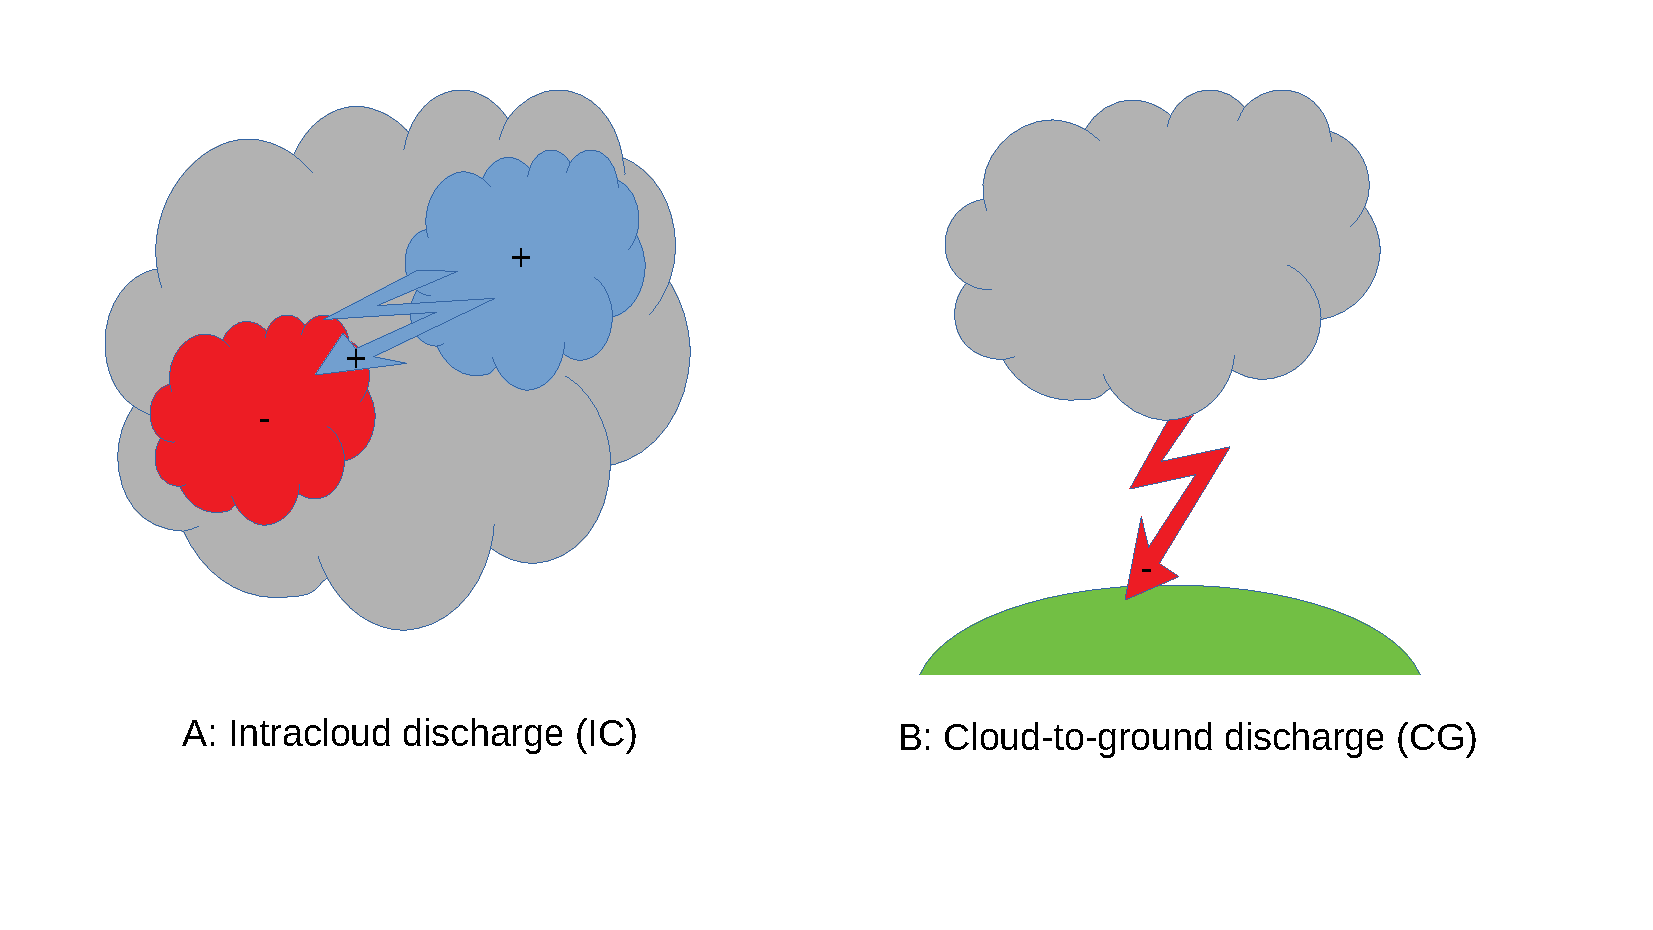
\includegraphics[width=\textwidth]{Figures/lyntyper.pdf}
    \caption{The two main categories of lightning. A shows an \acrfull{ic}, this could be between different storm cells or between different charge areas of the same storm cell. B shows a \acrfull{cg}, the polarity is defined by the charge change of earth. Negative cloud-to-ground (-CG) is defined by increase of negative charge at ground, and so positive cloud-to-ground (+CG) is defined by decrease of negative charge (increase in positive) at ground}
    \label{fig:lyntyper}
\end{figure}


\subsection{Winter lightning}
Winter lightning is a relatively well-studied phenomenon in Japan. Cold air from Siberia moves over the warm Tsushima current off the west coast of Japan, causing convection due to a strong temperature gradient between the cold air and the warm ocean. The supply of humidity from the seawater leads to formation of hydrometeors. The resulting convection has been shown to produce lightning strikes and thunderstorms during winter (\cite{michimoto2007}).

A similar phenomenon is observed off the west coast of Norway (e.g \cite{koeltzow2018}; \cite{march2016}). Cold air is moved from the Arctic to the Norwegian coast where the ocean is warmed by the North Atlantic Current. The resulting temperature gradient may give rise to  convection and subsequent electrification.

Both these phenomena lead to a convective and electrically active belt along the coasts, which is seen in the lightning climatologies for winter in both (\cite{koeltzow2018}; \cite{march2016})
 %This updraft and the creation of hydrometeors leads to an electrification that results in the aforementioned thunderstorms. 
 
\section{Helicopter Triggered Lightning}
A \acrlong{htl} is thought to be triggered by the helicopter's presence, causing there to be no need for lightning activity before or after the hit. This also means that a system that would create an \acrshort{htl} is harder to identify, as there are no warning signs in the form of thunder. 

The phenomenon is believed to be caused by the helicopter entering or coming close to an electrically charged part of a convective system.  This may be caused by several different mechanisms: The helicopter could be subject to a charge build-up during flight and then cause a discharge into the charged area of opposite polarity. However, given enough free charge in the cloud, the charged area could also discharge into the helicopter \textit{without} charge buildup in the helicopter.  Alternatively, the helicopter could induce a \acrshort{cg} by acting as part of the leader, see figure \ref{fig:triggertyper}. These different mechanisms are then analogous to \acrshort{ic} and \acrshort{cg}, respectively. 

A positively charged discharge is believed to cause more damage to helicopters than their negatively charged counterparts. The discharges to helicopters are also more often positive  (\cite{hardwick1999}).

\begin{figure}
    \centering
    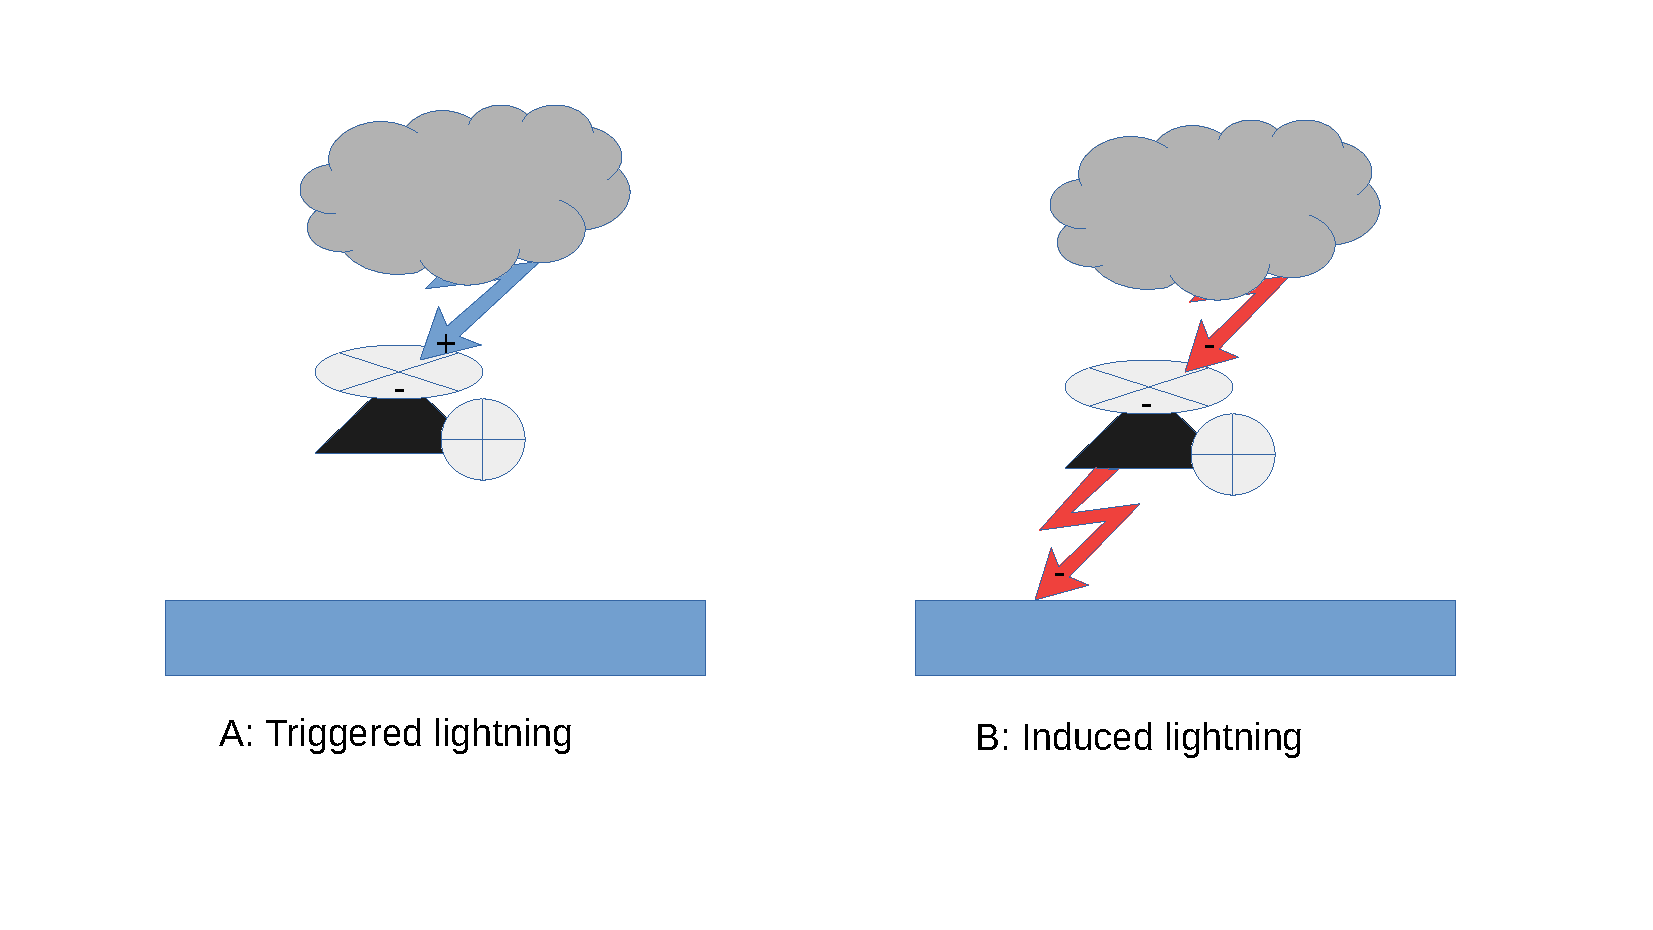
\includegraphics[width=\textwidth]{Figures/triggertyper.pdf}
    \caption{Illustration of different models for aircraft triggering. A shows the normal trigger situation, where the electrical discharge is grounded into the oppositely charged aircraft. B shows the situation where the aircraft is only acting as a pathway to the ground (Here ocean or land)}
    \label{fig:triggertyper}
\end{figure}

\section{Fixed Wing Triggered Lightning}

A \acrlong{fwtl} is also believed to be triggered by the presence of the aircraft, the main difference compared to \acrshort{htl} is that \acrshort{fwtl} is not solely a winter phenomenon. This is believed to be because planes fly higher in the atmosphere, and therefore will cross or enter the electrically charged part of the cloud.



